\documentclass[11pt]{article}
\usepackage[utf8]{inputenc}
\usepackage[T1]{fontenc}
\usepackage{amsmath}
\usepackage{amssymb}
\usepackage{multicol}
\usepackage{geometry}
\usepackage{tikz}
\usepackage{enumitem}
\usepackage{xcolor}
\usepackage{titlesec}

% Configurações de layout
\geometry{a4paper, left=1cm, right=1cm, top=0.5cm, bottom=1.2cm}
\setlength{\columnseprule}{0.4pt}

% Cores para títulos
\titleformat{\section}{\normalfont\Large\bfseries\color{blue}}{\thesection}{1em}{}
\titleformat{\subsection}{\normalfont\large\bfseries\color{red}}{\thesubsection}{1em}{}

\title{\textcolor{blue}{Terceiro Trimestre: Matemática
    \\Progressão Geométrica: Função Exponencial de Domínio Discreto}}
\author{Professor: Jefferson}
\date{}

\begin{document}

\maketitle
\vspace{-1cm}

\begin{center}
\large{Nome: \underline{\hspace{8cm}} \quad Turma: \underline{\hspace{3cm}}}
\end{center}

\begin{multicols}{2}

\section*{Habilidade:}

% CAIXA COLORIDA COM A HABILIDADE
\begin{tikzpicture}
\node[rectangle, 
      fill=purple!15, 
      rounded corners=5pt, 
      inner sep=10pt, 
      draw=purple!60!black, 
      thick,
      drop shadow={opacity=0.3}] (box) 
{
\begin{minipage}{0.75\linewidth}
\justifying
\small
\textbf{(EM13MAT508PE47)} Identificar e associar progressões geométricas (PG) a funções exponenciais de domínios discretos, para análise de propriedades, dedução de fórmulas e resolução de situações-problema em diversos contextos.
\end{minipage}
};
\end{tikzpicture}

\vspace{1mm}

\section*{1. Introdução à Progressão Geométrica (PG)}
Uma Progressão Geométrica é uma sequência numérica onde cada termo, a partir do segundo, é igual ao anterior multiplicado por uma constante chamada \textbf{razão} (q).

\subsection*{Exemplos de PG}
\begin{itemize}
\item $(2, 4, 8, 16, 32, \ldots)$ com $q = 2$
\item $(81, 27, 9, 3, 1, \ldots)$ com $q = \frac{1}{3}$
\item $(5, -10, 20, -40, 80, \ldots)$ com $q = -2$
\end{itemize}

\section*{2. Fórmula do Termo Geral: Progressão Geométrica}
Partindo da analogia:

\begin{align*}
a(1) &= a_1 \\
a(2) &= a_1 \cdot q \\
a(3) &= a_1 \cdot q^2 \\
a(4) &= a_1 \cdot q^3 \\
&\vdots \\
a(n) &= a_1 \cdot q^{n-1}
\end{align*}

\subsection*{Fórmula do Termo Geral}

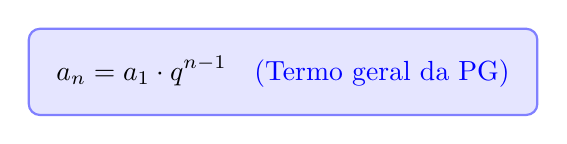
\begin{tikzpicture}
\node[rectangle, fill=blue!10, rounded corners, inner sep=10pt, draw=blue!50, thick] (box) {
$\displaystyle a_n = a_1 \cdot q^{n-1} \quad \text{\textcolor{blue}{(Termo geral da PG)}}$
};
\end{tikzpicture}

\vspace{5mm}

\textbf{Onde:}
\begin{itemize}
\item $\textcolor{red}{a_n}$ = termo geral
\item $\textcolor{red}{a_1}$ = primeiro termo
\item $\textcolor{red}{n}$ = posição do termo
\item $\textcolor{red}{q}$ = razão da PG
\end{itemize}

\subsection*{Exemplo}
Calcule o sexto termo da PG $(3, 6, 12, 24, \ldots)$

\textbf{Solução:}
\begin{align*}
a_1 &= 3,\quad q = \frac{6}{3} = 2 \\
a_6 &= 3 \cdot 2^{6-1} = 3 \cdot 2^5 = 3 \cdot 32 = 96
\end{align*}

\section*{3. Soma dos Termos de uma PG}

\subsection*{Fórmula da Soma}

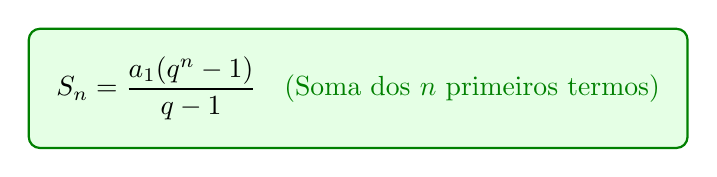
\begin{tikzpicture}
\node[rectangle, fill=green!10, rounded corners, inner sep=10pt, draw=green!50!black, thick] (box) {
$\displaystyle S_n = \frac{a_1(q^n - 1)}{q - 1} \quad \text{\textcolor{green!50!black}{(Soma dos $n$ primeiros termos)}}$
};
\end{tikzpicture}

\vspace{5mm}

\textbf{Onde:}
\begin{itemize}
\item $\textcolor{blue}{S_n}$ = soma dos $n$ primeiros termos
\item $\textcolor{blue}{a_1}$ = primeiro termo
\item $\textcolor{blue}{q}$ = razão da PG ($q \neq 1$)
\item $\textcolor{blue}{n}$ = número de termos
\end{itemize}

\subsection*{Dedução da Fórmula}
\begin{align*}
S_n &= a_1 + a_1q + a_1q^2 + \cdots + a_1q^{n-1} \\
qS_n &= a_1q + a_1q^2 + \cdots + a_1q^{n-1} + a_1q^n \\
\hline
qS_n - S_n &= a_1q^n - a_1 \\
S_n(q - 1) &= a_1(q^n - 1) \\
S_n &= \frac{a_1(q^n - 1)}{q - 1}
\end{align*}

\subsection*{Exemplo}
Calcule a soma dos 6 primeiros termos da PG $(3, 6, 12, 24, \ldots)$

\textbf{Solução:}
\begin{align*}
S_6 &= \frac{3(2^6 - 1)}{2 - 1} = \frac{3(64 - 1)}{1} = 3 \cdot 63 = 189
\end{align*}

\section*{4. PG como Função Exponencial Discreta}
Uma PG pode ser vista como uma função exponencial com domínio nos números naturais:

\[
f: \mathbb{N}^* \rightarrow \mathbb{R}
\]
\[
f(n) = a_1 \cdot q^{n-1}
\]

\subsection*{Comparação}

\scalebox{0.6}{

\begin{tabular}{|l|l|}
\hline
\textbf{Função Exponencial Contínua} & \textbf{PG (Função Exponencial Discreta)} \\
\hline
$f(x) = a \cdot b^x$, $x \in \mathbb{R}$ & $f(n) = a_1 \cdot q^{n-1}$, $n \in \mathbb{N}^*$ \\
\hline
Gráfico: curva exponencial contínua & Gráfico: pontos em curva exponencial \\
\hline
Taxa de crescimento proporcional ao valor atual & Razão de crescimento constante $q$ \\
\hline
\end{tabular}
}

\begin{center}
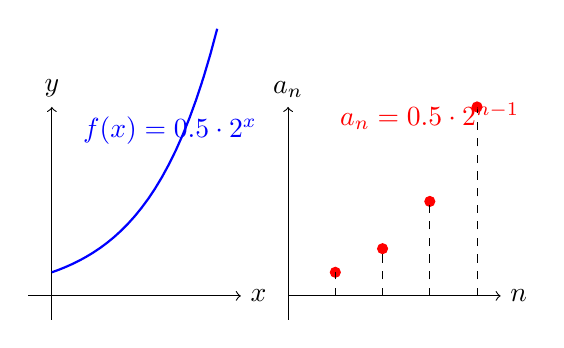
\begin{tikzpicture}[scale=0.6]
% Função exponencial contínua
\draw[->] (-0.5,0) -- (4,0) node[right]{$x$};
\draw[->] (0,-0.5) -- (0,4) node[above]{$y$};
\draw[blue, thick, domain=0:3.5] plot (\x, {0.5*(2^\x)});
\node[blue] at (2.5,3.5) {$f(x)=0.5 \cdot 2^x$};

% PG discreta
\draw[->] (5,0) -- (9.5,0) node[right]{$n$};
\draw[->] (5,-0.5) -- (5,4) node[above]{$a_n$};
\foreach \n in {1,2,3,4} {
    \filldraw[red] (5+\n,{0.5*(2^(\n-1)}) circle (3pt);
    \draw[dashed] (5+\n,0) -- (5+\n,{0.5*(2^(\n-1))});
}
\node[red] at (8,3.8) {$a_n=0.5 \cdot 2^{n-1}$};
\end{tikzpicture}
\end{center}

\section*{5. Análise de Propriedades}
\subsection*{Taxa de Crescimento Constante}
Em uma função exponencial $f(x) = a \cdot b^x$, a taxa de crescimento é proporcional ao valor atual.

Na PG:
\[
\frac{a_{n+1}}{a_n} = q \quad \text{(constante)}
\]

\subsection*{Propriedade Exponencial}
Tanto a função exponencial quanto a PG preservam:
\begin{itemize}
\item Multiplicatividade: $f(n+k) = f(n) \cdot q^k$
\item Crescimento acelerado (quando $q > 1$)
\item Decaimento exponencial (quando $0 < q < 1$)
\end{itemize}

\section*{6. Aplicação em Problemas}
\subsection*{Exemplo 1: Juros Compostos}
Um investimento de R\$ 1000,00 rende 10\% ao mês. Qual será o montante após 6 meses?

\textbf{Solução:}
\small{
\begin{align*}
a_1 &= 1000,\quad q = 1,10 \\
    a_6 &= 1000 \cdot (1,10)^{6-1} = 1000 \cdot 1,10^5 \\ 
    & \approx 1000 \cdot 1,61051 = R\$ 1610,51
\end{align*}
}

\subsection*{Exemplo 2: Crescimento Bacteriano}
Uma colônia de bactérias dobra a cada hora. Se inicialmente há 500 bactérias, quantas haverá após 8 horas?

\textbf{Solução:}
\begin{align*}
a_1 &= 500,\quad q = 2 \\
a_8 &= 500 \cdot 2^{8-1} = 500 \cdot 2^7 = 500 \cdot 128 = 64.000 \text{ bactérias}
\end{align*}

\section*{7. Exercícios de Progressão Geométrica}

\begin{enumerate}[leftmargin=*]

\item Determine o 8º termo da PG $(2, 6, 18, 54, \ldots)$

\item Numa PG, o 3º termo vale 20 e o 6º termo vale 160. Calcule:
\begin{enumerate}[label=\alph*)]
\item A razão da PG
\item O primeiro termo
\item A soma dos 8 primeiros termos
\end{enumerate}

\item Interpole 4 meios geométricos entre 2 e 486.

\item Calcule a soma dos 10 primeiros termos da PG $(1, 3, 9, 27, \ldots)$

\item Três números estão em PG. O produto deles é 216 e a soma é 21. Determine esses números.

\item (UFPE) Se o 4º termo de uma PG é 48 e o 7º termo é 384, qual é o 1º termo?

\item (ENEM) Uma população de bactérias triplica a cada hora. Se inicialmente há 200 bactérias, quantas haverá após 6 horas?

\item Dada a PG $(x+1, 3x, 9x-6)$, determine:
\begin{enumerate}[label=\alph*)]
\item O valor de x
\item A razão da PG
\item O oitavo termo
\end{enumerate}

\item Um carro sofre desvalorização de 15\% ao ano. Se hoje vale R\$ 40.000,00, quanto valerá daqui a 5 anos?

\item (UERJ) Uma bola é lançada de uma altura de 10m. A cada quique, ela atinge 70\% da altura anterior. Qual a distância total percorrida pela bola até o 5º quique?

\end{enumerate}

\section*{8. Exercícios de Associação PG-Função Exponencial}
\begin{enumerate}
\item Associe cada PG à sua função exponencial correspondente:
\begin{enumerate}[label=\alph*)]
\item $2, 4, 8, 16, \ldots$ \quad ( ) $f(n) = 3 \cdot 2^{n-1}$
\item $3, 6, 12, 24, \ldots$ \quad ( ) $f(n) = 2 \cdot 2^{n-1}$
\item $4, 8, 16, 32, \ldots$ \quad ( ) $f(n) = 2 \cdot 4^{n-1}$
\end{enumerate}

\item Dada a PG com $f(2) = 12$ e $f(5) = 96$, determine:
\begin{enumerate}[label=\alph*)]
\item A razão $q$
\item O termo inicial $a_1$
\item A expressão da função exponencial $f(n)$
\end{enumerate}

\item Um medicamento tem meia-vida de 6 horas. Se a dose inicial é 400mg, modele como:
\begin{enumerate}[label=\alph*)]
\item Função exponencial contínua
\item PG discreta (para intervalos de 6 horas)
\item Calcule a quantidade remanescente após 24 horas em ambos modelos
\end{enumerate}

\end{enumerate}

\end{multicols}

\end{document}
